\section{Следящая система управления положением звена.}

С увеличением сложности объекта управления более успешными становятся сложные, многокаскадные системы управления. Попытка внедрения функционала прохождения траектории или обхода препятствий непосредственно в алгоритм системы стабилизации или системы задания координат, хотя и может претендовать на достижения неких оптимальных показателей, представляется сомнительной с инженерной точки зрения, поскольку приводит к сильной связности алгоритмов управления, неочевидности поведения системы, требует трудоёмкой аналитической переработки при внесении изменений в функционал управления, повышает требования к квалификации работников технического сопровождения.

Разделив задачу управления на несколько слабо связанных задач, можно использовать каждое из них для введения уставки следующей. Так мы можем задавшись некоторыми ограничениями на динамические возможностями нашей системы, построить решение задачи траекторного управления достаточной точности, учитывающее обход препятствий всеми звеньями кинематической цепи без необходимости просчета временных функции кинематических координат $q_i(t)$. 

С другой стороны мы обеспечиваем решение задачи координатного управления, чтобы все уставки $P_i(t)$ выданные для каждого момента времени траекторным алгоритмом выполнялись с необходимой точностью.

Такое разбиение позволяет координатному решателю не заботиться о геометрических ограничениях ввиду того, что они учтены траекторным решателем, а траекторный решатель может расчитывать управление траектории в удобных для этой задачи координатах, поскольку не связан необходимостью физического управления изделием.   

\begin{center}
  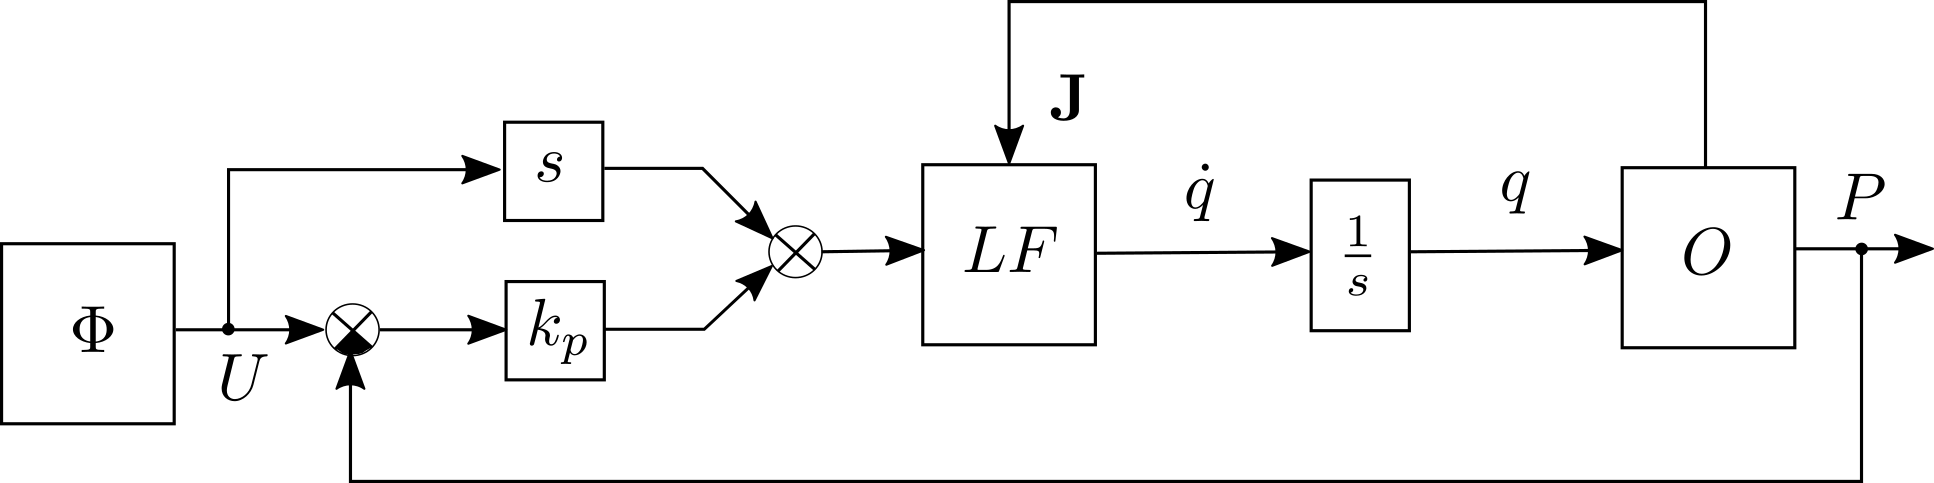
\includegraphics[width=\textwidth,height=\textheight,keepaspectratio]{ctrsyst.png}
  \captionof{figure}{Структурная схема следящей системы.}
  \label{}
\end{center}

Получив решение обратной скоростной задачи мы получили возможность синтезировать управления заданного 6-скоростью объекта положения звена. Однако, обычно, целью позиционера является управлением положением звена, а не его скоростью.

Прямое решение задачи управления положением через интеграл скоростного управления, очевидно, очень быстро приведет к накоплению вычислительной ошибки.

Чтобы исключить вычислительную ошибку зададимся модельным положением управляемого звена. Пусть задача траекторного управления вырабатывает уставку в виде текущих объектов положения $U(t)$ и скорости $\dot{U}(t)$.

Используем объект уставки как основной сигнал управления (прямое управление), а объект положения для вычисления ошибки $E(t)$ в цепи обратной связи.

Тогда система управления будет отрабатывать управляющее воздействие $\dot{U}(t)$, замешивая в него с небольшим коэффициентом ошибку по положению $E(t)$.

Компенсация $E(t)$ вносится в форме 6-вектора положения взвешенного на соответствующий коэффициент усиления.

Если сумирование компоненты линейной скорости уставки и взвешенного сигнала ошибки положения не вызывает вопросов в силу линейности преобразований координат и линейных скоростей, то сумирование компонент угловой скорости и взвешенных компонент вектора поворота необходимо обосновать.

Возьмём вектор компенсации $\Omega_e$ сонаправленный сигналу ошибки углового положения $\rho_e$ и равный по модулю $K|\rho_e|$, где $K$ размерный коэффициент приведения.
Разложим вектор компенсации $\Omega_e$ на аксиальную и тангенсальную к вектору $\omega_u$ направления.   

Тогда сумарный вектор угловой скорости будет иметь вид 
\begin{equation}
\omega = |\omega_u + \omega_e^{tang}|\bar{t} + |\omega_e^{norm}|\bar{n}
\end{equation} 
Тангенсальная компонента $\omega_e^{tang}$ прямо корректирует модуль $\omega_u$, ускоряя или замедляя воздействие исходя из текущей ошибки. Компонент $\omega_e^{norm}$ подворачивает звено к ориентации модельного положения. В силу ортогональности управления по тангенсальному и нормальному ортам можно считать независимым при достаточно малом вычислительном шаге.

Надо отметить, что ошибка углового положения более неприятна для системы в целом, поскольку приводит к повороту базиса и переносу ошибки на компоненты линейного положения. Соответственно, следует либо устанавливать высокие требования к динамической точности такой системы, либо осуществлять предобработку сигнала управления путём переноса в связанный базис. 

На текущий момент доказательством устуйчивости построенной СУ является вычислительный эксперимент. Аналитической исследование устойчивости системы управления выходит за рамки настоящего изложения. Наработка методов анализа устойчивости систем управления объектами работающими в трехмерном пространстве является перспективным направлением развития настоящей работы. 

Следует также отметить, что может быть построена система управления исключительно по сигналу $E(t)$ без прямого управления по $U(t)$. Такая система имеет лучшую устойчивость и не имеет проблемы переноса ошибки углового положения на компоненты линейного, но имеет худшее быстродействие и может иметь статическую ошибку в режиме движения с ненулевой скоростью.